\documentclass[twocolumn]{aastex631}
\received{\today}
\shorttitle{Giant Planet Formation}
\graphicspath{{figures/}}

\usepackage{lipsum}
\usepackage{physics}
\usepackage{multirow}
\usepackage{xspace}
\usepackage{natbib}
\usepackage{fontawesome5}
\usepackage{xcolor}
\usepackage{wrapfig}
\usepackage[figuresright]{rotating}

% remove indents in footnotes
\usepackage[hang,flushmargin]{footmisc} 

\newcommand{\todo}[1]{{\color{red}{[TODO: #1}]}}
\newcommand{\needcite}{{\color{magenta}{(needs citation)}}}
\newcommand{\placeholder}[1]{{\color{gray} \lipsum[#1]}}

% custom function for adding units
\makeatletter
\newcommand{\unit}[1]{%
    \,\mathrm{#1}\checknextarg}
\newcommand{\checknextarg}{\@ifnextchar\bgroup{\gobblenextarg}{}}
\newcommand{\gobblenextarg}[1]{\,\mathrm{#1}\@ifnextchar\bgroup{\gobblenextarg}{}}
\makeatother

\begin{document}

\title{{\huge Giant Planet Formation}\\\vspace{0.15cm}ASTR558 Final Project}

% affiliations
\newcommand{\UW}{Department of Astronomy, University of Washington, Seattle, WA, 98195}

\author[0000-0001-6147-5761]{T. Wagg}
\affiliation{\UW}

\correspondingauthor{Tom Wagg}
\email{tomwagg@uw.edu}

\begin{abstract}
    \textbf{Background and Context:} There are currently two main theories for the formation of giant planets, core accretion and direct collapse. Core accretion can explain the formation of most planets but for those far from their host star, direct collapse is needed to explain their existence on the timescale of the age of the Universe.
\end{abstract}

\keywords{}

\section{Key Concepts}

In this section, we explain the key concepts behind the two main theories of giant planet formation.

\subsection{Core Accretion}

\subsubsection{How does it work?}

At its simplest level, core accretion is where a central rocky core is formed and then accretes gas until it reaches a critical core mass and forms a giant planet \citep{Pollack+1996}. This general process is illustrated in the left planet of Figure~\ref{fig:formation_diagram}.

The formation occurs in three phases, which can be seen in Figure~\ref{fig:planet_growth}. In the first phase, the planet is formed primarily of solid material and continuously accretes planetessimals at a higher rate than gas until the planet clears its ``feeding zone'', marking the end of the first phase. At this point the core of the planet has formed and now the planet slowly accretes gas in an envelope. This gas is accreted from a sphere of radius \citep{Bodenheimer+2013}
\begin{equation}
    R = \min \{ R_{\rm Bondi}, R_{\rm Hill} \}
\end{equation}
where $R_{\rm Bondi}$ is the Bondi radius, defining the maximum distance inside which gas can be bound to the core and $R_{\rm Hill}$ is the Hill radius, defining the radius in which the main gravitational influence is the planet. See Appendix~\ref{app:maths} for a derivation of these radii.

The third phase of core accretion begins as the planetary core exceeds the critical core mass, resulting in rapid envelope contraction that leads to fast accretion of gas and thus planet mass growth. This finals results in a giant planet.

\begin{figure}
    \centering
    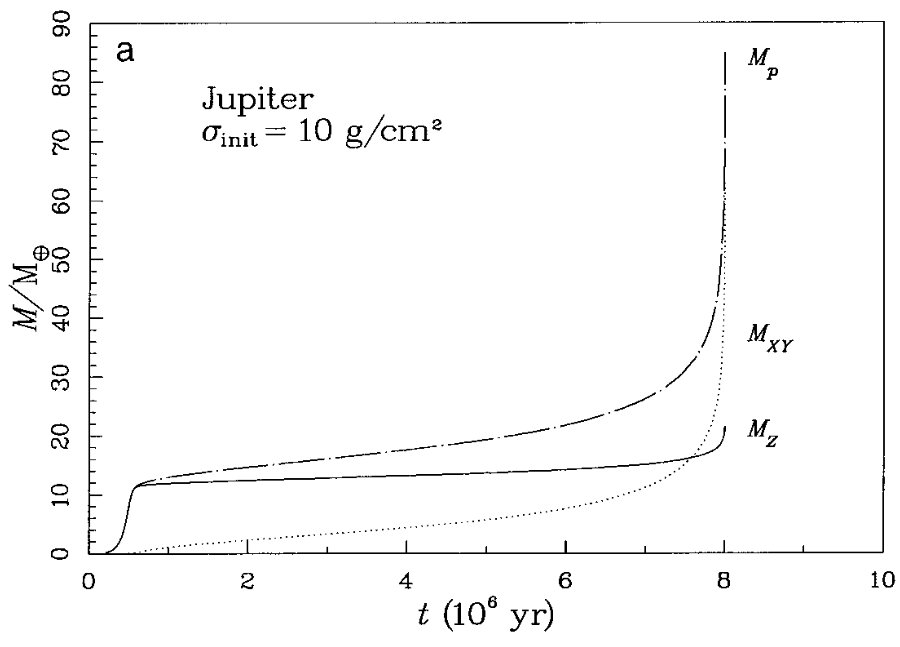
\includegraphics[width=\columnwidth]{pollack_fig_1.png}
    \caption{Figure 1 of \citet{Pollack+1996}. Planet mass as a function of time in which the three phases of core accretion are evident (rapid early accretion in phase 1, low accretion rate in the middle is phase 2, final rapid accretion is phase 3). The different curves show the masses of different compositions.}
    \label{fig:planet_growth}
\end{figure}

\subsubsection{Critical core mass}
\subsubsection{The end of accretion}

\subsubsection{Timescale limits}

\subsection{Direct Collapse}

\subsubsection{How does it work?}

\subsubsection{Migration}

\begin{figure}
    \centering
    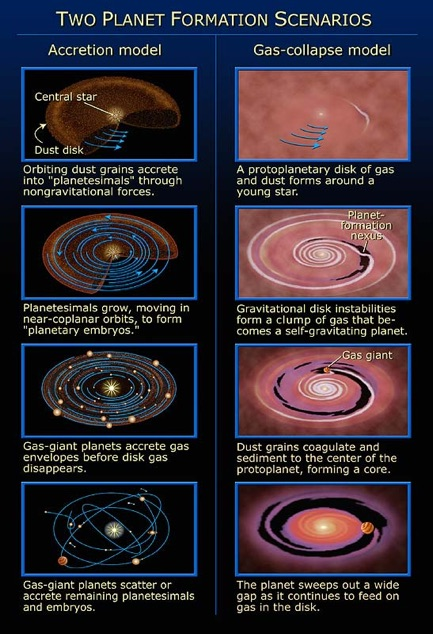
\includegraphics[width=\columnwidth]{channels_illustration.jpg}
    \caption{An illustration of different giant planet formation channels. (Credit: NASA and A. Feild (STScl))}
    \label{fig:formation_diagram}
\end{figure}

\section{Recent Research}

\section{Unsolved Questions}

\begin{itemize}
    \item Challenges with direct collapse \citep{Forgan+2013}
    \item Core accretion doesn't account for compositional gradients \citep{D'Angelo+2018}
\end{itemize}

\bibliographystyle{aasjournal}
\bibliography{paper}{}

\appendix

\section{Derivation of Bondi and Hill Radii}\label{app:maths}

\todo{}

\end{document}